\documentclass{book}[a5paper]
\usepackage[a5paper]{geometry}
\usepackage[utf8]{inputenc}
\usepackage{amsmath}
\usepackage{amsthm}
\usepackage{amssymb}
\usepackage[font=small,labelfont=bf]{caption}
\usepackage{wrapfig}
\usepackage{enumitem}

\usepackage{xfp}
\usepackage{pgfplots, pgfplotstable}
\usetikzlibrary{pgfplots.units}
\pgfplotsset{compat=1.16}

\usepackage{tikz}
\usepackage{float}

% Speed up the compile time for TIKZ
%\usepgfplotslibrary{external}
%\tikzexternalize

\newcommand{\placeholder}{[Insert Section Here]}

\newtheorem{theorem}{Theorem}[section]
\newtheorem{corollary}{Corollary}[theorem]
\newtheorem{lemma}[theorem]{Lemma}
\newtheorem*{remark}{Remark}


% Exercise section 
\newlist{exercise}{enumerate}{5}
\setlist[exercise]{label*=\arabic*.,ref=\arabic*,before={\subsection*{Exercises}}}
\let\ex\item

% Style to select only points from #1 to #2 (inclusive)
\pgfplotsset{select coords between index/.style 2 args={
    x filter/.code={
        \ifnum\coordindex<#1\def\pgfmathresult{}\fi
        \ifnum\coordindex>#2\def\pgfmathresult{}\fi
    }
}}

\title{Linear Regression}
\author{Zachary Ross}
\date{November 2019}

\begin{document}

\section{Real Value Prediction}

For this section, our motivation is to construct an algorithm whose focus is
predicting a value. That is, we want a \emph{prediction function} which takes an
input, called a \emph{feature}, and produces some numeric reponse, called a
\emph{scalar response}, between $-\infty$ and $\infty$. As with the rest of
machine learning and with life itself, we \emph{learn} using experiences, or
features.

% TODO: Include information on application

\subsection{Linear Regression}

% TODO: Site sources:
% - https://www.kaggle.com/c/house-prices-advanced-regression-techniques/data

The main focus of this section is determining a real number
that is associated with some other number. In a linear sense, we are finding
a continuous function that takes in one number and spits out another using
previously gathered data. So the question is, how do we form this function?


\begin{figure}[t!]
\centering
    \begin{tikzpicture}
        \selectcolormodel{gray}
        \begin{axis}[
                title = {HOUSE PRICES CORRELATED WITH PLOT AREA},  % whatever name you want
                xlabel = {Plot Area in 1,000 ft$^2$},
                ylabel = {House Price in \$100,000},
                tick label style={/pgf/number format/fixed},
                scaled y ticks = false,
                scaled x ticks = false,
                yticklabel={
                    \fpeval{\tick / 100000}               % Divide the y coordinate/1000
                },
                xticklabel={
                    \fpeval{\tick / 1000}               % Divide the y coordinate/1000
                },
            ]
            \addplot[
                only marks,
                select coords between index={1}{50},
                ] table[col sep=comma]{linreg_houseprice.csv};
        \end{axis}
    \end{tikzpicture}
    \caption{List of plot areas and selling prices for houses in Ames, Iowa.
    Looking at these kind of plots, we can try to find correlations in the data
    that help us predict what future houses may cost in that market.}
    \label{fig:hp}
\end{figure}

The scatterplot in Figure \ref{fig:hp} shows a bit of housing data from Ames,
Iowa. There is a positive correlation when comparing each plot area with its
corresponding price, showing us that as plot area increases, so does the house
price. We can ascribe this relationship to a variable $\theta_1$. That is,
$\theta_1$ is the price per square foot of plot area
($\frac{\text{price}}{\text{ft}^2}$). Additionally, we can establish a
\emph{base price} to this correlation. That is, we can instantiate some other
variable, call it $\theta_0$, which acts as an offset for the housing prices. In
context, this offset can be considered the starting price for houses in Ames,
such that any plot will cost the base price of \$100,000 plus the price per
square foot.

Examining these properties sets us up to form a hypothesis for how house prices
are determined.  If we let $\theta = \begin{pmatrix}\theta_0 \\
\theta_1\end{pmatrix}$ be a vector of the associated prices with the base price
as $\theta_0$ and price per ft$^2$ as $\theta_1$, and let $X^{(i)}$ be the plot
area for the $i$th feature in the training set $X$, the equation
\begin{equation}
    hypothesis(\theta, X^{(i)}) = \theta_0 + \theta_1X^{(i)}
\end{equation}
should ideally give us the price for $X^{(i)}$. The key word in the last
sentence is \emph{ideally} since the hypothesis function will only give us 100\%
accuracy when all the data in the data set lies exactly on the line formed by
the hypothesis. This would mean that each square foot of plot area would cost
the exact same amount at every house you check. However optimal this is, it is
generally not the case. Instead, we look to maximize the accuracy of this
function or otherwise minimize the \emph{error}. We do this by altering the
prices in $\theta$.


We begin measuring the error of our hypothesis by comparing it with the
previously collected data.  An intuitive way for measuring the  error of the
hypothesis would be by measuring the shortest distance between the value it
predicts and the recorded value since this, in a literal sense, tells us how far
off our prediction was from the result. 

\begin{wrapfigure}{O}{0.5\textwidth}
    \centering
    \resizebox{0.5\textwidth}{!}{
        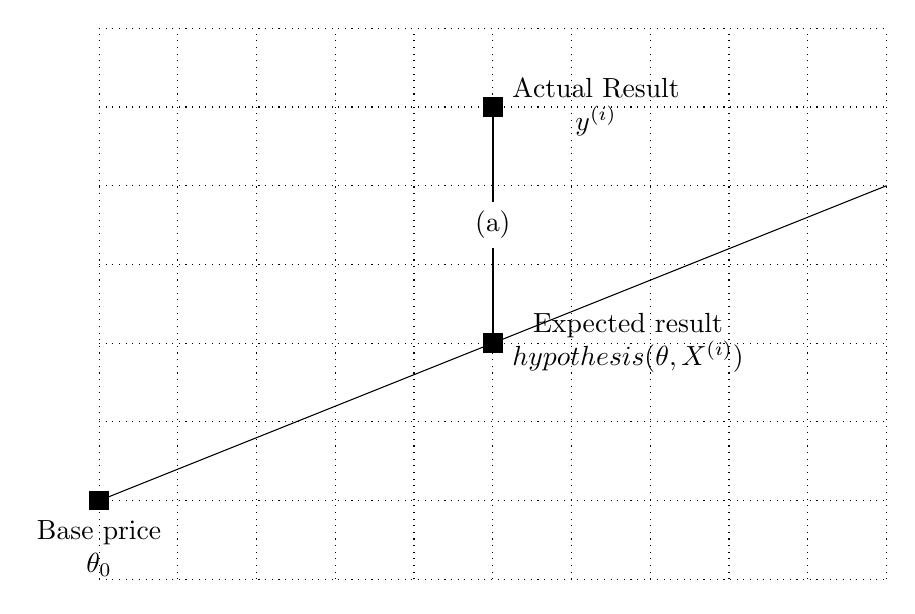
\begin{tikzpicture}[every label/.style={align=center}]
            \node[draw, fill=black, label=right:{Actual Result \\ $y^{(i)}$}] (v1) at (5,6) {};
            \node[draw, fill=black, label=right:{Expected result \\ $hypothesis(\theta, X^{(i)})$}] (v2) at (5,3) {};
            \node[draw, fill=black, label=below:{Base price \\ $\theta_0$}] (v3) at (0,1) {};

            \draw[dotted] (0,0) grid (10,7);
            \draw (0,1) -- (10,5);
            \draw[thick] (v1) -- (v2) node [midway, fill=white] {(a)};
        \end{tikzpicture}
    }
    \caption{Visual representation of the distance between expected and actual
    results.}
    \label{fg:err}
\end{wrapfigure}

We see how this is found in Figure \ref{fg:err} by first examining the case for
a single feature. The hypothesis function predicts a result for $X^{(i)}$, which
corresponds to some base price plus the cost of the lot area in our example from
earlier. We then compare this to the original result at $y^{(i)}$ by finding the
distance between these two points, which is precisely the norm of these two
points. The distance we are trying to find is the length of the line marked by
(a). Since these two points have the same $x$ coordinate, those coordinates will
cancel out and so it suffices to find the distance between their $y$
coordinates. We know the distance between any two points to be $\| point_1 -
point_2 \|$ or equivalently $(point_1 - point_2)^2$.  Putting this all together,
we define the square error function to be
\begin{equation}
    error(\theta, X^{(i)}, y^{(i)}) = (hypothesis(\theta, X^{(i)}) - y^{(i)})^2
\end{equation}
. Note that the value output by $error$ will always be positive since the the
square of any number is positive or zero.

We then need a way to measure the total error generated by the hypothesis
function across all of the features. This total error generated is called the
\emph{cost} of our hypothesis function. For this, a good estimate of our cost is
the \emph{mean squared error (MSE)} which is described in more detail in Section
[Insert Loss Function section here]. So if we let $m$ be the number of features
in $X$, the cost function
\begin{equation}
    Cost(\theta, X, y) = \frac{1}{m}\sum_{i=1}^m error(\theta, X^{(i)}, y^{(i)})
\end{equation}
will give us a good estimate for how well $\theta$ is performing in
the hypothesis. Expanded out, this is equivelent to
\begin{equation}
    Cost(\theta, X, y) = \frac{1}{m}\sum_{i=1}^m (\theta_0 + \theta_1X^{(i)} -
    y^{(i)})^2
\end{equation}
.

\begin{figure}[htp!]
    \centering
    \pgfplotsset{ticks=none}
    \begin{minipage}{.3\textwidth}
        \centering
        \resizebox{\textwidth}{!}{
            \begin{tikzpicture}

                \selectcolormodel{gray}
                \begin{axis}[
                    ]
                    \addplot[
                        only marks,
                        select coords between index={1}{50},
                    ] table[col sep=comma]{linreg_houseprice.csv};
                \end{axis}
            \end{tikzpicture}
        }
        (a)
    \end{minipage}
    \begin{minipage}{.3\textwidth}
        \centering
        \resizebox{\textwidth}{!}{
            \begin{tikzpicture}

                \selectcolormodel{gray}
                \begin{axis}[
                    ]
                    \addplot[
                        only marks,
                        select coords between index={1}{50},
                    ] table[col sep=comma]{linreg_houseprice.csv};
                \end{axis}
            \end{tikzpicture}
        }
        (b)
    \end{minipage}
    \begin{minipage}{.3\textwidth}
        \centering
        \resizebox{\textwidth}{!}{
            \begin{tikzpicture}

                \selectcolormodel{gray}
                \begin{axis}[
                    ]
                    \addplot[
                        only marks,
                        select coords between index={1}{50},
                    ] table[col sep=comma]{linreg_houseprice.csv};
                \end{axis}
            \end{tikzpicture}
        }
        (c)
    \end{minipage}
    \caption{}
    \label{fg:weights1}
\end{figure}

\begin{exercise}
    \ex Why do we take the mean square error instead of the total square error?
    \ex Compare and contrast the benefits of different loss functions with the
    MSE in regards to linear regression.
\end{exercise}

\end{document}
